%----------------------------------------------------------------------------
\chapter{The paper, chapter by chapter}\label{app:chapters}
%----------------------------------------------------------------------------
The chapter files contain headings, orange notes linking here, running-example boxes, one item per tagged list, and the figure and table stubs needed by the lint. This chapter explains each heading: what reviewers score, the paragraph's beat (\cref{app:writing:spine}) and worked examples using \exname. Read the matching section before drafting. Copy examples from \texttt{guide/05-chapter-by-chapter.tex}, removing \texttt{guide:} from copied labels: \texttt{req:guide:offline} becomes \texttt{req:offline}.

This is the fictional paper from the mind map in \cref{fig:mindmap}. Approaches A to D, measurements and results illustrate completed items; they do not describe a real system.

\paragraph{What the reviewer scores.} The review sheet scores five criteria, A to E; \cref{app:tdk:sheet} names them and quotes their top steps. For A, the sheet sets a 30--35 page limit and recommends that reviewers deduct 1 point per 3 pages outside it. Support four claims throughout the paper, as explained below. Each section quotes the steps below the top that cost a chapter points.
\begin{description}[noitemsep]
  \item[Relevance (C)] The topic matters now.
  \item[Non-triviality (C and D/1)] Solving the problem requires deep or scientific knowledge beyond a textbook recipe or reuse of known solutions.
  \item[Novelty (D/1)] Full marks for a solution that is new at least in Hungary or does not exist yet; an incremental improvement earns 3--4 of 5.
  \item[Correctness (D/2)] Every result is backed and checkable.
\end{description}
Criterion A is scored on the whole paper.

\paragraph{What a skimming reviewer reads.} A busy reviewer may read only what the skim view keeps (\cref{app:lifecycle:reviewers}), such as tagged items (C1, REQ1, AS1, SG1, \dots), and register prose only by its length. Headings marked \skimmark{} contain items visible in this reading. If a section is unmarked, also express its claim in a marked item, a caption or the heading.

%----------------------------------------------------------------------------
\section{Introduction}\label{app:chapters:intro}
%----------------------------------------------------------------------------
\textbf{Criteria C and E.} A reviewer who reads only the introduction and its leading figure should be able to say what you did and why it matters.
\textbf{Relevance:} open with why the problem matters now and to whom.
\textbf{Non-triviality:} show why the obvious solutions fail.
\textbf{Novelty:} state the contributions as checkable claims.

\textbf{In the sheet's words.} The bottom of E (\cref{app:tdk:sheet}) names what this chapter must contain, together with the evaluation: \enquote{0: teljesen hiányzik -- ha a dolgozat bevezetése hiányos (tématerület áttekintése, problémafelvetés, fő kontribúció kimondása) ÉS az eredmények gyakorlati validálása, értékelése is hiányzik ill. hibás}.

\subsection{Context}\label{app:chapters:context}
\guidebeat{why the field matters now}{a trend, a regulation or an incident, cited}{not yet introduced}{the problem}
Every abbreviation goes through \texttt{\textbackslash gls}, as in \gls{vc}, which spells it out on first use; declare it in \texttt{content/glossary.tex}, together with the paper's notation and terms, unless the common glossary (\cref{tab:glossary-common}) already has it.

\subsection[Problem]{Problem\skimmark}\label{app:chapters:problem}
\guidebeat{the concrete problem, ending in a one-sentence problem statement}{the running example}{introduced here: who the actors are, what they want to do, and what goes wrong}{the requirements}
Introduce the example in two or three sentences: the actors, their goal and what goes wrong. Choose a scenario simple enough to follow across chapters but rich enough to show every requirement.
\begin{runningexample}
A university issues a diploma to a graduate as a verifiable credential, and later revokes it because the degree was withdrawn. An employer checks the diploma during hiring and accepts it: its copy of the revocation status is a day old.
\end{runningexample}

\subsection[Requirements]{Requirements\skimmark}\label{app:chapters:requirements}
\guidebeat{what a solution must do}{one requirement per failure of the example; they are the rows of the gap matrix and the yardstick of the evaluation}{the part of the scenario each requirement comes from}{the gap}
State each requirement as a checkable property needed by the example. Usually, existing approaches trade one requirement against the others.
\begin{requirements}
  \item\label{req:guide:timely} \textbf{Timely revocation.} Every verifier sees a revocation within $\delta$ of its submission.
  \item\label{req:guide:offline} \textbf{Offline checks.} A verifier checks a credential without contacting its issuer.
  \item\label{req:guide:private} \textbf{Holder privacy.} A check tells nobody, the issuer included, which credential was checked.
\end{requirements}

\subsection{Gap, in brief}\label{app:chapters:introgap}
\guidebeat{that no existing approach meets the requirements together; the full comparison comes after the evaluation (\cref{ch:related}), so this paragraph carries the novelty claim on its own}{the closest approaches, cited}{what the closest approach does with the example, and where it fails}{the contributions}
Name the closest approaches and the requirements each sacrifices. Here, asking the issuer at every check is timely but neither offline nor private; offline lists are private but a day stale.

\subsection[Leading figure]{Leading figure\skimmark}\label{app:chapters:leading-figure}
\textbf{Criterion B/1} assesses figures like this. \Cref{app:writing:figure} says what it shows; \cref{app:writing:captions,app:writing:figures} cover its caption and drawing.

\textbf{In the sheet's words.} The step below the top of B/1 (\cref{app:tdk:sheet}) is \enquote{2: átlagos (a dolgozat megfelelő számú ábrát és táblázatot tartalmaz, ám azok több esetben nem jól átgondoltak vagy rossz minőségűek)}.

\begin{figure}[!ht]
  \centering
  \begin{tikzpicture}[
      node distance=6mm and 10mm,
      col/.style={draw, rounded corners, minimum width=38mm, minimum height=26mm, align=center, font=\small},
      part/.style={ours, rounded corners=1pt, minimum width=34mm, minimum height=7mm, align=center, font=\footnotesize},
      lbl/.style={font=\small\bfseries, above=1mm}]
    \node[col, problem]   (problem) {A revoked diploma\\[1mm]\footnotesize is accepted, because\\\footnotesize the status is a day old};
    \node[part, right=12mm of problem, yshift=9mm] (c1) {C1: Registry model};
    \node[part, below=1.5mm of c1] (c2) {C2: Ledger registry};
    \node[part, below=1.5mm of c2] (c3) {C3: Evaluation};
    \node[draw=none, fit=(c1)(c3), inner sep=2mm] (approach) {};
    \node[col, result, right=of approach] (result) {Rejected within $\delta$\\[1mm]\footnotesize offline, and the issuer\\\footnotesize never learns who asked};
    \node[lbl] at (problem.north)  {Problem};
    \node[lbl] at (approach.north) {This work};
    \node[lbl] at (result.north)   {Evaluation};
    \draw[-Stealth, thick] (problem) -- (approach);
    \draw[-Stealth, thick] (approach) -- (result);
  \end{tikzpicture}
  \caption{The leading figure combines the problem, contributions and headline result. The problem is red, all components of this work are blue, and the result is green.}
  \label{fig:guide:overview}
\end{figure}

\subsection[Contributions]{Contributions\skimmark}\label{app:chapters:contributions}
\guidebeat{what this work claims, as checkable items with pointers to their support}{the chapters behind each contribution}{the leading figure shows the example solved}{the structure of the paper}
Give each contribution its own item and supporting chapter reference: the theoretical result (model, formalisation, algorithm or protocol and its guarantees), the technical result (tool, system or artifact), and the evaluation.
\begin{contributions}
  \item\label{c:guide:model} \textbf{Registry model.} A formal model of revocation registries, and a proof that verifiers never accept a credential revoked more than $\delta$ ago (\cref{ch:approach}).
  \item\label{c:guide:registry} \textbf{Ledger registry.} A registry on a permissioned ledger where a check reads one accumulator witness, without asking the issuer, archived with its tests (\cref{ch:implementation}).
  \item\label{c:guide:eval} \textbf{Evaluation.} Correctness on the model and the scenario, scalability up to 10\,000 issuers, and robustness under node failures and load spikes (\cref{ch:evaluation}).
\end{contributions}

\subsection{Structure}\label{app:chapters:structure}
Describe each chapter in one sentence, in reading order. The introduction already contains this paragraph; update its chapter names when you rename the files' headings. A dependency graph of the paper can stand in for the list (\cref{app:writing:depgraph}).

%----------------------------------------------------------------------------
\section{Background}\label{app:chapters:background}
%----------------------------------------------------------------------------
\textbf{Criterion B/2.} Cite current research and industrial solutions, not only course material.
\textbf{Non-triviality:} explain the concepts needed for the difficult parts of \cref{ch:approach}. Cite textbook material without deriving it again.
\textbf{Nothing of yours here.} Limit the background to prior knowledge and cite every statement. The chapter boundary should clearly separate prior work from your contribution.
\textbf{A companion paper.} When a TDK paper of the same year supplies what your approach builds on, restate the part this paper needs here, condensed, and introduce it as the companion paper's work without a citation (\cref{app:tdk:companion}). It is the only part of this chapter without a reference.

\textbf{In the sheet's words.} The scale for B/2 starts at \enquote{0: egyetemi tananyag (a dolgozat kizárólag egyetemi tankönyveket idéz kapcsolódó szakirodalomként)}, and its step 1 is well-known industrial practice from web pages (\cref{app:writing:refs}); this chapter must already cite above that.

\subsection[First concept]{First concept\skimmark}\label{app:chapters:first-concept}
\guidebeat{the first concept the approach relies on; notation is defined once, here}{a definition and a citation}{the example expressed with this concept}{the second concept}
Name the section after its concept. Define it precisely enough for later chapters, then use its vocabulary to restate the introductory scenario in the box.
\begin{runningexample}[in terms of verifiable credentials]
The diploma is a verifiable credential: the university is its \gls{issuer}, the graduate its \gls{holder}, and the employer a \gls{verifier}. The revocation is a second statement by the issuer, and the verifier must see it too.
\end{runningexample}
\begin{definition}[Verifiable credential]\label{def:guide:vc}
A \emph{verifiable credential} is a set of claims about a subject, signed by its issuer, that its holder can present to any verifier without the issuer taking part.
\end{definition}

\subsection{Second concept}\label{app:chapters:second-concept}
\guidebeat{the second concept}{a definition and a citation}{the example expressed with this concept}{the approach}
For the registry, explain the permissioned ledger used to store revocations: its guarantees about history and the cost of appending.

%----------------------------------------------------------------------------
\section{Approach}\label{app:chapters:approach}
%----------------------------------------------------------------------------
\textbf{Criteria D/1 and D/2 (0--10 together).} Present your theoretical contribution, such as a model, formalisation, algorithm or protocol, and its guarantees. Put technical contributions in \cref{ch:implementation}. Name this chapter after your method.
\textbf{Correctness:} every claim needs a proof, a mechanised proof, or a measurement; state assumptions explicitly.
\textbf{Novelty:} separate what is new from what you adopted from the literature.
\textbf{Non-triviality:} name the hard part and explain why the simple design does not work.
\textbf{Describe here, evaluate later.} Explain the approach and its guarantees objectively. Assess how well it works in the evaluation, where you can support that assessment with evidence.

\subsection[Overview]{Overview\skimmark}\label{app:chapters:overview}
\guidebeat{how the approach works end to end}{the architecture figure}{the example walked through the figure, component by component}{the model}
Walk through the figure in the example box, showing which component handles each step and what it produces.
\begin{runningexample}[through the approach]
The university revokes the diploma at the registry service, which removes it from the accumulator and appends the new value, signed and timed, to the ledger. When the graduate presents the diploma with its witness, the employer's verifier library checks the witness against the newest signed value it holds, which must be younger than $\delta$. The revoked diploma's witness no longer verifies, and the diploma is rejected.
\end{runningexample}

\begin{figure}[!ht]
  \centering
  \begin{tikzpicture}[
      node distance=8mm and 14mm,
      comp/.style={draw, rounded corners, fill=blue!8, minimum width=28mm, minimum height=10mm, align=center, font=\small},
      ext/.style={comp, prior, dashed}]
    \node[ext]  (user) {Issuer};
    \node[comp, ours, right=of user] (core) {Registry service\\\footnotesize(contribution C2)};
    \node[comp, prior, right=of core] (store) {Permissioned ledger};
    \node[comp, ours, below=of core] (check) {Verifier library\\\footnotesize(contribution C2)};
    \draw[-Stealth] (user) -- node[above, font=\footnotesize]{revoke} (core);
    \draw[-Stealth] (core) -- node[above, font=\footnotesize]{append} (store);
    \draw[-Stealth] (core) -- node[right, font=\footnotesize]{signed value} (check);
    \begin{scope}[on background layer]
      \node[draw, dotted, inner sep=3mm, fit=(core)(store)(check), label={[font=\footnotesize]above right:System boundary}] {};
    \end{scope}
  \end{tikzpicture}
  \caption{Registry architecture. Blue marks this work; grey marks reused or external parts. The issuer is outside the system, and the ledger is an existing product.}
  \label{fig:guide:architecture}
\end{figure}
Replace the approach chapter's figure stub with your architecture (\cref{fig:guide:architecture}). Keep your components blue.

\subsection{Model or design}\label{app:chapters:model}
\guidebeat{the formal model or the design decisions}{each decision with the alternative rejected and why}{the example as an instance of the model}{the threat model}
Name this section after the model. For the registry, describe the valid credentials as an accumulator, its signed and timed ledger values, the holder's witness that a credential is still in it, and the diploma removed by revocation.

\subsection{Threat model and guarantees}\label{app:chapters:threat-model}
\guidebeat{who the adversary is and what it can do, who is trusted, which cryptographic assumptions hold, what is out of scope, and what the approach guarantees under all that}{a proof, a mechanised proof, or a measurement in the evaluation for every guarantee}{the attack on the example that the threat describes}{the implementation}
\textbf{Give the threat model all four parts below.} Reviewers of security work look for each.
\textbf{Adversary:} state what it controls (network, participants, keys), its capabilities (reading, replaying, reordering, dropping, forging with its keys) and its limits. Use a standard model where appropriate: Dolev--Yao for a protocol, honest-but-curious or malicious participants, or a computational adversary with a security parameter for a cryptographic construction.
\textbf{Trust:} which parties are assumed honest, and what happens if one is not.
\textbf{Cryptographic assumptions:} list the primitives and required properties as assumptions that proofs can reference.
\textbf{Out of scope:} state here which attacks you do not address, and why, so reviewers can distinguish exclusions from omissions.
State guarantees as \enquote{under these assumptions, against this adversary, the following holds}. The evaluation's correctness table (\cref{tab:guide:correctness}) records how each was checked.

\subsection[Adversary]{Adversary\skimmark}\label{app:chapters:adversary}
In the example box, show each adversary and the guarantee that stops it.
\begin{threats}
  \item\label{thr:guide:holder} \textbf{Malicious holder.} A holder who keeps a witness from before the revocation and presents it again.
  \item\label{thr:guide:network} \textbf{Network adversary.} Controls the network between the registry and the verifiers, in the Dolev--Yao model: reads, replays, delays and drops messages.
\end{threats}
\begin{runningexample}[under attack]
The graduate presents the diploma with last week's witness (\cref{thr:guide:holder}); a network adversary holds back the newest accumulator value from the employer (\cref{thr:guide:network}). Both fail on \cref{g:guide:stale}: the old witness verifies only against a value older than $\delta$, and the employer accepts no older value.
\end{runningexample}

\subsection[Attacks]{Attacks\skimmark}\label{app:chapters:attacks}
If you name concrete attacks, give each a row in \cref{tab:guide:attacks}: the adversary, defence and residual risk. Otherwise omit this paragraph and table.
\begin{table}[!ht]
  \centering
  \caption{Registry attacks, adversaries, defences and residual risks.}
  \label{tab:guide:attacks}
  {\small
  \begin{tabularx}{\linewidth}{>{\raggedright\arraybackslash}X l >{\raggedright\arraybackslash}X >{\raggedright\arraybackslash}X}
    \toprule
    \textbf{Attack} & \textbf{By} & \textbf{Stopped by} & \textbf{Residual risk} \\
    \midrule
    A revoked diploma is presented with an old witness & \cref{thr:guide:holder} & \cref{g:guide:stale} & none \\
    A held-back value hides a fresh revocation & \cref{thr:guide:network} & \cref{asm:guide:clock}, \cref{g:guide:stale} & revocations younger than $\delta$ \\
    An accumulator value or a witness is forged & \cref{thr:guide:holder} & \cref{asm:guide:sig} & none \\
    \bottomrule
  \end{tabularx}
  }
\end{table}

\subsection[Trust and cryptographic assumptions]{Trust and cryptographic assumptions\skimmark}\label{app:chapters:assumptions}
\begin{assumptions}
  \item\label{asm:guide:sig} \textbf{Sound signatures and accumulator.} The registry's signature scheme is existentially unforgeable under chosen-message attack, and no witness exists for a credential removed from the accumulator.
  \item\label{asm:guide:clock} \textbf{Bounded drift.} The clocks of the registry and the verifiers differ by less than $\delta$.
  \item\label{asm:guide:operator} \textbf{Honest-but-curious operator.} The registry operator follows the protocol but reads everything it sees.
\end{assumptions}

\subsection{Out of scope}\label{app:chapters:out-of-scope}
For the registry, the excluded attacks are denial of service and compromised holder devices.

\subsection[Guarantees]{Guarantees\skimmark}\label{app:chapters:guarantees}
Prove each guarantee here or check it in the evaluation.
\begin{guarantees}
  \item\label{g:guide:stale} \textbf{Bounded staleness.} Under \cref{asm:guide:sig,asm:guide:clock,asm:guide:operator}, against \cref{thr:guide:holder,thr:guide:network}, a verifier rejects every credential revoked more than $\delta$ before the check.
\end{guarantees}

You may also list derived requirements: properties the design needs to satisfy its guarantees, such as owner-only writes or replay protection. Check each by test or proof in the evaluation. These do not belong in the gap matrix and may be listed in the implementation chapter instead.
\begin{derivedrequirements}
  \item\label{dr:guide:owner} \textbf{Owner-only revocation.} Only a credential's issuer can append its revocation.
\end{derivedrequirements}

\begin{lemma}[Fresh values]\label{lem:guide:fresh}
Under \cref{asm:guide:sig,asm:guide:clock}, every accumulator value a verifier accepts was signed by the registry less than $\delta$ before the check.
\end{lemma}
\begin{theorem}[Bounded staleness]\label{thm:guide:stale}
\Cref{g:guide:stale} holds against \cref{thr:guide:holder,thr:guide:network}.
\end{theorem}
\begin{proof}
By \cref{lem:guide:fresh}, the accepted value is at most $\delta$ old, and by \cref{asm:guide:operator} it excludes every credential revoked before it; by \cref{asm:guide:sig}, a credential it excludes has no witness.
\end{proof}

%----------------------------------------------------------------------------
\section{Implementation}\label{app:chapters:implementation}
%----------------------------------------------------------------------------
\textbf{Criteria D/1 and D/2.} Explain your technical contributions. Avoid a class-by-class description. Rename this chapter after what you built if helpful. If the implementation is not a contribution itself, make it a section of \cref{ch:approach} and use the saved pages for evaluation.
\textbf{Novelty:} identify what you built, whether a tool, system, prototype, integration or dataset. Distinguish it from reused libraries, frameworks and tools.
\textbf{Non-triviality:} explain design decisions and obstacles to a straightforward implementation.
\textbf{Correctness:} give readers enough detail to assess and reproduce the evaluation. Include architecture, reasons for technology choices and the Zenodo code archive. Cite its concept DOI and name the results tag beside it (\cref{app:zenodo}).

\textbf{In the sheet's words.} D/2 drops to \enquote{2: kérdéses (színvonalas kidolgozás, de egyes részletekben kisebb szakmai hibák vannak, vagy egyes eredmények helyessége kérdéses / egyáltalán nem ellenőrizhető)} when a result cannot be checked: the archived code and the reproduction command are what make it checkable.

\subsection[Overview]{Overview\skimmark}\label{app:chapters:impl-overview}
\guidebeat{what was built and how it realises the approach}{the components of the architecture figure mapped to code; the archived artifact}{the example as the system's input or configuration}{the design decisions}
Map architecture components to code and cite the archive. Fill in the citation and repository link already in your file. The example box should show the implementation's input: a configuration, model or test case.
\begin{runningexample}[as input]
The scenario is a test case: one issuer, one diploma, a revocation at $t = 0$, and checks at $t = 1$, $2$ and $3$\,s. It passes when every check after $\delta = 2$\,s rejects the diploma.
\end{runningexample}

\subsection{Design decisions}\label{app:chapters:design-decisions}
\guidebeat{the engineering choices, and the problems a straightforward build runs into}{each decision with the alternative rejected and why}{where the example exposed the problem}{the key technical contribution}
For the registry, explain why verifiers keep signed accumulator values: reading the ledger directly would require a node at every verifier. Also explain why $\delta$ is a parameter rather than a constant.

\subsection[The key technical contribution]{The key technical contribution\skimmark}\label{app:chapters:key-contribution}
\guidebeat{the part of the implementation that did not exist before}{the one listing that shows it, and the tests that cover it}{the example processed by it, step by step}{the evaluation}
Name the section after your contribution and show the snippet that explains its key idea.
\begin{lstlisting}[caption={The verifier's check: the accumulator value is signed and younger than $\delta$, and the holder's witness shows the credential is still in it.}, label={lst:guide:key}]
fun accept(cred, witness, acc, now):
  return verify(registryKey, acc.signature)
     and now - acc.signedAt <= DELTA
     and memberOf(cred.id, witness, acc.value)
\end{lstlisting}

%----------------------------------------------------------------------------
\section{Evaluation}\label{app:chapters:evaluation}
%----------------------------------------------------------------------------
\textbf{Criteria E (0--8) and D/2.}
\textbf{Correctness:} give the setup, versions and repetitions needed to check every number. D/2 penalises unverifiable results.
\textbf{Novelty:} compare against the closest existing approach named in the introduction; the related-work chapter then places the results in the wider literature.
\textbf{Beyond small examples:} E awards 7--8 points only for scalability and robustness measurements beyond small examples that support use in an industrial setting. \Cref{tab:guide:eval-tracks} applies this to formal and analysis topics.

\textbf{In the sheet's words.} D/2 gives \enquote{3--4: jó (színvonalas kidolgozás, de esetleg egyes eredmények helyessége nincs kellőképpen alátámasztva)} when a result is reported without the setup that supports it, and E gives \enquote{1--2: nagyon hiányos -- ha a dolgozat bevezetése hiányos (tématerület áttekintése, bemutatása, problémafelvetés, fő kontribúció kimondása) VAGY az eredmények értékelése hiányzik ill. aránytalanul kis méretű vagy hibás} when the evaluation stops at small examples. An evaluation that goes beyond them but is incomplete or imprecise earns \enquote{3--4: pontatlan -- ha a dolgozat bevezetése megfelelő és a dolgozatban szerepel az eredmények kis mintapéldákon túlmenő értékelése is, de az utóbbi hiányos, pontatlan} or \enquote{5--6: pontos, de hiányos}.

\textbf{Three kinds of work, one chapter.} The examples below primarily describe a measured system (track S). Formal work (track F: Tamarin or ProVerif models, Lean or Coq proofs, model checking) and benchmarked analysis tools (track T: detectors, static analysers, generators) answer the same three questions with different evidence. Use \cref{tab:guide:eval-tracks}, the alternative figures and tables, and the track F and T research questions in the source to adapt the chapter.

\begin{table}[!ht]
  \centering
  \caption{Evaluation evidence and presentation by track: S for measured systems; F for protocol models, mechanised proofs and model checking; T for analysis tools evaluated on benchmarks.}
  \label{tab:guide:eval-tracks}
  {\small
  \begin{tabularx}{\linewidth}{>{\raggedright\arraybackslash}p{0.13\linewidth} >{\raggedright\arraybackslash}X >{\raggedright\arraybackslash}X >{\raggedright\arraybackslash}X}
    \toprule
    & \textbf{S: system} & \textbf{F: formal} & \textbf{T: analysis tool} \\
    \midrule
    Setup & Hardware, software versions, workloads, repetitions, the rerun command & Prover and version, heuristics and oracles, time limit, machine; which parts of the model are hand-written and which generated & Benchmark origin and size, how the ground truth was built, tool versions, the rerun command \\
    \addlinespace
    Correctness (\cref{rq:guide:correct}) & Test suite and model-checked properties per requirement; the running example before and after (\cref{tab:guide:correctness}, \cref{fig:guide:example-trace}) & Every property of the threat model proved, or an attack found: per lemma, proved, falsified with the trace, or timed out; the attack on the running example reconstructed (\cref{tab:guide:correctness}, one row per lemma) & Precision and recall against the ground truth, every false positive and false negative explained (\cref{tab:guide:precision}); the running example's verdict (\cref{fig:guide:example-trace}) \\
    \addlinespace
    Scalability (\cref{rq:guide:scale}) & Throughput and latency as the input grows (\cref{fig:guide:scalability}) & Verification time and memory as the model grows: sessions, agents, bound, lemma count; where the prover times out, and what helper lemmas buy (\cref{fig:guide:scalability-formal}) & Analysis time as the input grows: circuit size, lines, model elements; the largest real instance it handles (\cref{fig:guide:scalability}) \\
    \addlinespace
    Robustness (\cref{rq:guide:robust}) & Faults, load spikes and parameter sensitivity, with degradation and recovery (\cref{tab:guide:robustness}, \cref{fig:guide:robustness}) & The properties re-verified under a stronger adversary and with each assumption dropped: which hold, which break and how (\cref{tab:guide:robustness-formal}) & Thresholds and parameters varied, mutated or adversarial inputs, benchmark instances from another source (\cref{tab:guide:robustness}) \\
    \bottomrule
  \end{tabularx}
  }
\end{table}

\subsection[Research questions]{Research questions\skimmark}\label{app:chapters:research-questions}
Use three research questions, one for each evaluation section below.
\begin{rqlist}
  \item\label{rq:guide:correct} \textbf{Correctness.} Does the registry reject every revoked credential, in the scenario and in the model, against both adversaries?
    % Track F: Does the model satisfy every property of the threat model, and does it find the known attacks?
    % Track T: Does the tool find the real instances in the benchmark, and only those?
  \item\label{rq:guide:scale} \textbf{Scale.} How do the latency of a check and the registry's throughput grow with the number of issuers?
    % Track F: How do verification time and memory grow with the size of the model, and where does the prover stop?
    % Track T: How does analysis time grow with input size, and what is the largest real instance it handles?
  \item\label{rq:guide:robust} \textbf{Robustness.} How does the registry behave when a ledger node fails, under a burst of checks, and as $\delta$ varies?
    % Track F: Which properties survive a stronger adversary and each dropped assumption, and how do the others break?
    % Track T: How do the results change under parameter changes, mutated inputs, and a benchmark from another source?
\end{rqlist}

\subsection{Setup}\label{app:chapters:setup}
\guidebeat{how the measurements were made, so that each can be checked}{hardware, software versions, workloads, repetitions, the rerun command}{the example as the base workload, scaled up for the scalability question}{the results}
For the registry: one 8-core virtual machine, four ledger nodes, synthetic issuer sets of 10 to 10\,000 issuers with 100 credentials each, 10 runs per point with fresh sets, and the command that reruns them.

\subsection{Artifact availability}\label{app:chapters:artifact-availability}
Archive code, models and measurement scripts on Zenodo. We require that all numbers in the chapter come from one tagged version, such as \texttt{v1.0.0}, and that \texttt{just reproduce} regenerates its figures and tables (\cref{app:zenodo}).

\subsection[Correctness (RQ1)]{Correctness (RQ1)\skimmark}\label{app:chapters:correctness}
\guidebeat{that the approach is correct on the example and on every requirement case}{test, proof or model-checking results}{the scenario's outcome, before and after}{scalability}
\textbf{Show correctness in two ways.} In \cref{tab:guide:correctness}, list how each guarantee and requirement was checked for your work and the baseline: a proof (Tamarin, Lean, \dots), model checking or tests. Adapt the rows to your work. Formal topics use proofs and counterexamples; empirical topics use test and benchmark results; analysis tools add \cref{tab:guide:precision}. Then show the example's outcome in \cref{fig:guide:example-trace}, comparing the baseline's failure with your result. Use a sequence chart for protocols or another suitable before-and-after diagram.
\begin{runningexample}[solved]
The employer's check now rejects the diploma 2\,s after the university revokes it, without asking the university, where the baseline accepted it for a day (\cref{fig:guide:example-trace}).
\end{runningexample}

\begin{table}[!ht]
  \centering
  \caption{Checks of each guarantee and requirement against the introduction's list-based baseline. \gapyes{} means proved or passed, \gappartial{} partial, and \gapno{} a counterexample or failure.}
  \label{tab:guide:correctness}
  {\small
  \begin{tabularx}{\linewidth}{>{\raggedright\arraybackslash}p{3.2em} >{\raggedright\arraybackslash}X >{\raggedright\arraybackslash}p{6em} c c r}
    \toprule
    & \textbf{Property} & \textbf{Checked by} & \textbf{This work} & \textbf{Baseline} & \textbf{Time} \\
    \midrule
    \ref{g:guide:stale} & Bounded staleness, as a lemma (\cref{thm:guide:stale}) & Tamarin & \gapyes & \gapno & 41\,s \\
    \ref{req:guide:timely} & Revocation test cases & test suite & \gapyes\,42/42 & \gappartial\,30/42 & 3\,s \\
    \ref{req:guide:offline} & Checks with the issuer unreachable & test suite & \gapyes\,20/20 & \gapyes\,20/20 & 1\,s \\
    \ref{req:guide:private} & The issuer cannot link two checks & Tamarin & \gapyes & \gapno & 380\,s \\
    \bottomrule
  \end{tabularx}
  }
\end{table}

\begin{table}[!ht]
  \centering
  \caption{Track T supplement to \cref{tab:guide:correctness}: precision and recall by benchmark family against ground truth. Explain every false positive and false negative in the text.}
  \label{tab:guide:precision}
  {\small
  \begin{tabularx}{\linewidth}{>{\raggedright\arraybackslash}X r r r r r r r}
    \toprule
    \textbf{Benchmark family} & \textbf{Instances} & \textbf{TP} & \textbf{FP} & \textbf{FN} & \textbf{Precision} & \textbf{Recall} & \textbf{Baseline recall} \\
    \midrule
    Hand-written cases from the introduction & 12 & 12 & 0 & 0 & 1.00 & 1.00 & 0.75 \\
    Mutated real instances & 40 & 37 & 2 & 3 & 0.95 & 0.93 & 0.60 \\
    Real instances from another source & 25 & 21 & 1 & 4 & 0.95 & 0.84 & 0.52 \\
    \bottomrule
  \end{tabularx}
  }
\end{table}

\begin{figure}[!ht]
  \centering
  \tikzset{lifeline/.style={dashed, gray}, role/.style={draw, rounded corners, fill=blue!8, minimum width=12mm, inner sep=2pt, font=\footnotesize}, msg/.style={-Stealth, font=\footnotesize}}
  \newcommand{\lifelines}{%
    \foreach \x/\n in {0/Issuer, 2.3/Holder, 4.6/Verifier, 6.9/Registry} {%
      \node[role] at (\x, 0) {\n}; \draw[lifeline] (\x, -0.3) -- (\x, -3.4);}%
    \draw[msg] (0, -0.8) -- node[above] {issue $c$} (2.3, -0.8);
    \draw[msg] (0, -1.4) -- node[above, pos=0.82] {revoke $c$} (6.9, -1.4);
    \draw[msg] (2.3, -2.0) -- node[above] {present $c$} (4.6, -2.0);}
  \begin{subfigure}[b]{0.49\linewidth}
    \centering
    \begin{tikzpicture}
      \lifelines
      \draw[msg] (4.6, -2.6) -- node[above] {check (stale)} (6.9, -2.6);
      \node[font=\footnotesize\bfseries, text=red!70!black] at (4.6, -3.7) {accepts $c$};
    \end{tikzpicture}
    \caption{Baseline: the revoked credential is accepted.}\label{fig:guide:example-trace-baseline}
  \end{subfigure}\hfill
  \begin{subfigure}[b]{0.49\linewidth}
    \centering
    \begin{tikzpicture}
      \lifelines
      \draw[msg] (4.6, -2.6) -- node[above] {check (current)} (6.9, -2.6);
      \node[font=\footnotesize\bfseries, text=green!45!black] at (4.6, -3.7) {rejects $c$};
    \end{tikzpicture}
    \caption{This work: the verifier sees the revocation and rejects the credential.}\label{fig:guide:example-trace-ours}
  \end{subfigure}
  \caption{The employer's check of revoked diploma $c$, before and after, as a sequence chart.}
  \label{fig:guide:example-trace}
\end{figure}

\FloatBarrier
\subsection[Scalability (RQ2)]{Scalability (RQ2)\skimmark}\label{app:chapters:scalability}
\guidebeat{how the cost grows with the input}{the scalability figure}{the example multiplied to $n$ participants or items}{robustness}
Explain what grows, how fast and where the limit lies. Put the better result higher on the plot: use a metric where higher is better (\cref{fig:guide:scalability-throughput}), or reverse the axis when lower is better (\cref{fig:guide:scalability-time}).

\begin{figure}[!ht]
  \centering
  \begin{subfigure}[b]{0.48\linewidth}
    \centering
    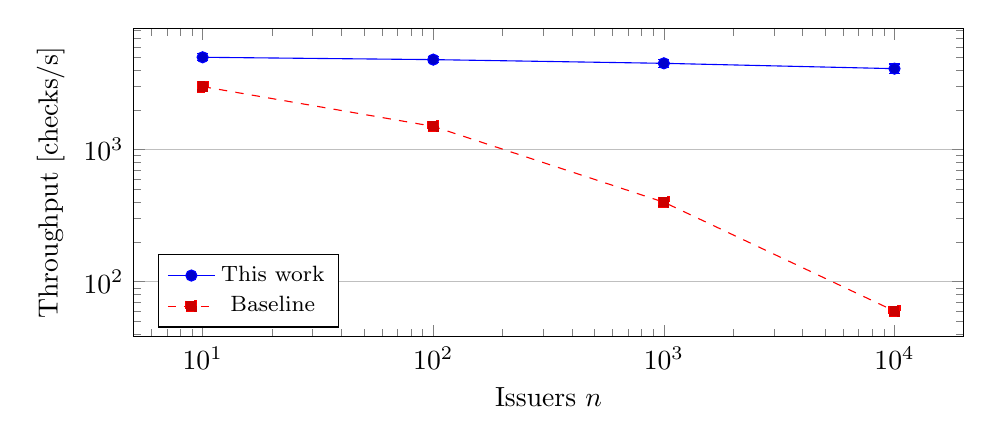
\begin{tikzpicture}
      \begin{axis}[width=\linewidth, height=55mm, xlabel={Issuers $n$}, xmode=log, ymode=log, ymajorgrids, legend style={font=\footnotesize}, ylabel={Throughput [checks/s]}, legend pos=south west]
        \addplot+[mark=*, error bars/.cd, y dir=both, y explicit]
          coordinates {(10,5000) +- (0,300) (100,4800) +- (0,250) (1000,4500) +- (0,300) (10000,4100) +- (0,350)};
        \addlegendentry{This work}
        \addplot+[mark=square*, dashed]
          coordinates {(10,3000) (100,1500) (1000,400) (10000,60)};
        \addlegendentry{Baseline}
      \end{axis}
    \end{tikzpicture}
    \caption{Throughput; higher is better.}\label{fig:guide:scalability-throughput}
  \end{subfigure}\hfill
  \begin{subfigure}[b]{0.48\linewidth}
    \centering
    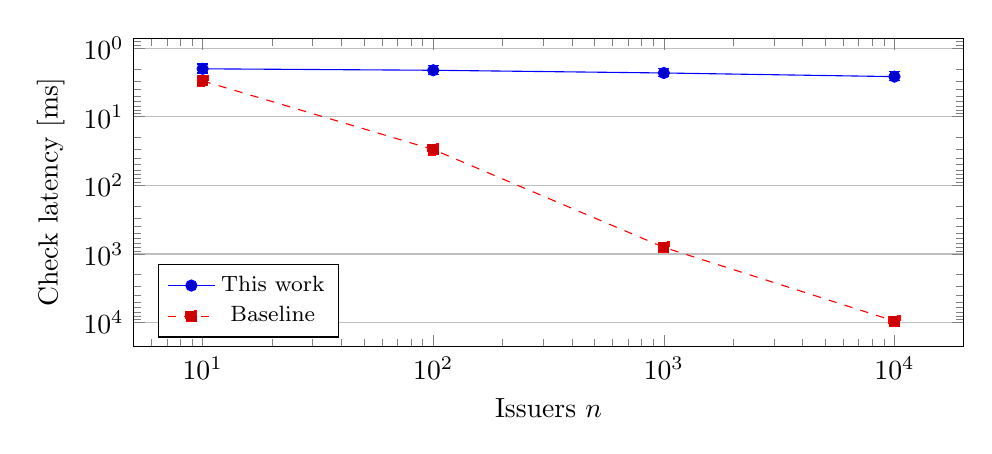
\begin{tikzpicture}
      \begin{axis}[width=\linewidth, height=55mm, xlabel={Issuers $n$}, xmode=log, ymode=log, ymajorgrids, legend style={font=\footnotesize}, ylabel={Check latency [ms]}, y dir=reverse, legend pos=south west]
        \addplot+[mark=*, error bars/.cd, y dir=both, y explicit]
          coordinates {(10,2) +- (0,0.3) (100,2.1) +- (0,0.3) (1000,2.3) +- (0,0.3) (10000,2.6) +- (0,0.4)};
        \addlegendentry{This work}
        \addplot+[mark=square*, dashed]
          coordinates {(10,3) (100,30) (1000,800) (10000,9500)};
        \addlegendentry{Baseline}
      \end{axis}
    \end{tikzpicture}
    \caption{Latency with a reversed axis: lower values appear higher.}\label{fig:guide:scalability-time}
  \end{subfigure}
  \caption{Performance as issuer count grows, with better results higher in both panels. Means of 10 runs with fresh issuer sets; error bars show one standard deviation.}
  \label{fig:guide:scalability}
\end{figure}

\begin{figure}[!ht]
  \centering
  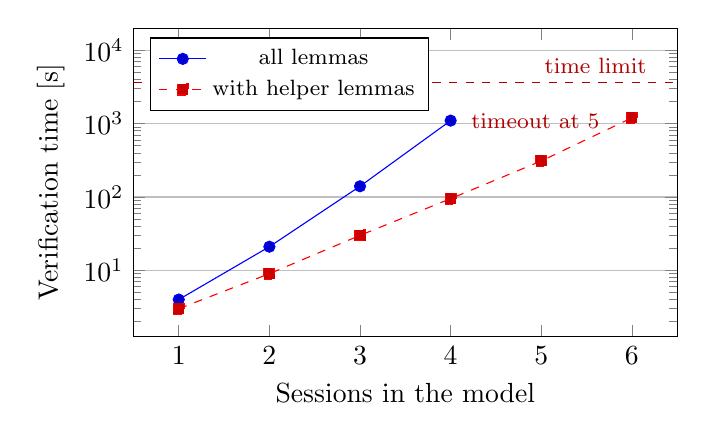
\begin{tikzpicture}
    \begin{axis}[width=0.7\linewidth, height=55mm, xlabel={Sessions in the model}, ylabel={Verification time [s]}, ymode=log, ymajorgrids, legend style={font=\footnotesize}, legend pos=north west, xmin=0.5, xmax=6.5, xtick={1,...,6}, ymax=20000]
      \draw[dashed, red!70!black] (axis cs:0.5,3600) -- (axis cs:6.5,3600) node[pos=0.85, above, font=\footnotesize] {time limit};
      \addplot+[mark=*] coordinates {(1,4) (2,21) (3,140) (4,1100)};
      \addlegendentry{all lemmas}
      \addplot+[mark=square*, dashed] coordinates {(1,3) (2,9) (3,30) (4,95) (5,310) (6,1200)};
      \addlegendentry{with helper lemmas}
      \node[font=\footnotesize, text=red!70!black, anchor=west] at (axis cs:4.12,1100) {timeout at 5};
    \end{axis}
  \end{tikzpicture}
  \caption{Track F alternative to \cref{fig:guide:scalability}: verification time as the model grows, including the time limit and where the prover stops. Use your model's size parameter: sessions, agents, a bounded-check limit or lemma count.}
  \label{fig:guide:scalability-formal}
\end{figure}

\subsection[Robustness analysis (RQ3)]{Robustness analysis (RQ3)\skimmark}\label{app:chapters:robustness}
\guidebeat{how the system behaves when its assumptions are stressed: faults, attacks, load spikes, parameter changes}{the robustness table, with the setup of each perturbation}{the example under attack}{the threats to validity}
\textbf{Robustness is required in addition to scalability} for the top of criterion E (\cref{app:chapters:evaluation}, \cref{app:tdk:sheet}).
\textbf{Track S:} deliberately perturb the system. Report each perturbation and outcome in \cref{tab:guide:robustness}. Use \cref{fig:guide:robustness} to show degradation and recovery during faults, and sensitivity to the main parameter.
\textbf{Track F:} use \cref{tab:guide:robustness-formal} to report each property under a stronger adversary and with each assumption dropped. Show which properties hold, which fail and the attacks that break them.
\textbf{Track T:} adapt \cref{tab:guide:robustness} to the tool. Vary thresholds and parameters around their defaults. Test mutated or adversarial inputs, including deliberately injected bugs, and use benchmark instances from a source other than the development data.

\begin{table}[!ht]
  \centering
  \caption{Registry behaviour under each perturbation, with its purpose, expected and observed results, and recovery.}
  \label{tab:guide:robustness}
  {\small
  \begin{tabularx}{\linewidth}{>{\raggedright\arraybackslash}p{0.2\linewidth} >{\raggedright\arraybackslash}X >{\raggedright\arraybackslash}p{0.16\linewidth} >{\raggedright\arraybackslash}p{0.16\linewidth} >{\raggedright\arraybackslash}p{0.12\linewidth}}
    \toprule
    \textbf{Perturbation} & \textbf{What it tests} & \textbf{Expected} & \textbf{Observed} & \textbf{Recovery} \\
    \midrule
    Fault injection & One of four ledger nodes crashes during a burst of checks & checks go on, revocations wait & as expected, revocations 3.1\,s late & 12\,s \\
    Adversarial input & \Cref{thr:guide:holder} replays a week-old witness, 500 times & all rejected & all rejected & none needed \\
    Load spike & 10$\times$ the nominal check rate for 60\,s & latency within one round trip & p99 at 1.8$\times$ nominal & immediate \\
    Parameter sensitivity & The ledger timeout varied around its default & graceful & see \cref{fig:guide:robustness-sensitivity} & none needed \\
    \bottomrule
  \end{tabularx}
  }
\end{table}

\begin{table}[!ht]
  \centering
  \caption{Track F alternative to \cref{tab:guide:robustness}: recheck each property under a stronger adversary and after dropping each assumption. \gapyes{} means proved, \gapno{} an attack with its trace in the appendix, and \gappartial{} a timeout.}
  \label{tab:guide:robustness-formal}
  {\small
  \begin{tabularx}{\linewidth}{l >{\raggedright\arraybackslash}X *{4}{>{\centering\arraybackslash}p{0.13\linewidth}}}
    \toprule
    & \textbf{Property} & \textbf{Base threat model} & \textbf{Registry key leaked} & \textbf{\ref{asm:guide:clock} dropped} & \textbf{Weaker signatures} \\
    \midrule
    \ref{g:guide:stale} & Bounded staleness (\cref{thm:guide:stale}) & \gapyes & \gapno & \gapno & \gappartial \\
    \ref{req:guide:private} & Holder privacy & \gapyes & \gapyes & \gapyes & \gapyes \\
    \bottomrule
  \end{tabularx}
  }
\end{table}

\begin{figure}[!ht]
  \centering
  \begin{subfigure}[b]{0.48\linewidth}
    \centering
    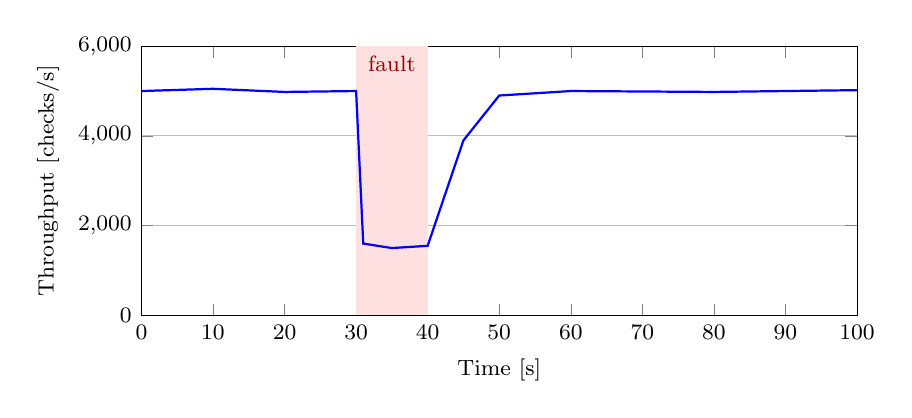
\begin{tikzpicture}
      \begin{axis}[width=0.88\linewidth, height=50mm, xlabel={Time [s]}, ylabel={Throughput [checks/s]}, ymin=0, ymax=6000, xmin=0, xmax=100, ymajorgrids, font=\footnotesize]
        \fill[red!12] (axis cs:30,0) rectangle (axis cs:40,6000);
        \node[font=\footnotesize, text=red!60!black] at (axis cs:35,5600) {fault};
        \addplot[mark=none, thick, blue] coordinates {(0,5000) (10,5050) (20,4980) (30,5000) (31,1600) (35,1500) (40,1550) (45,3900) (50,4900) (60,5000) (80,4980) (100,5020)};
      \end{axis}
    \end{tikzpicture}
    \caption{Degradation and recovery when a ledger node fails between 30 and 40\,s.}\label{fig:guide:robustness-fault}
  \end{subfigure}\hfill
  \begin{subfigure}[b]{0.48\linewidth}
    \centering
    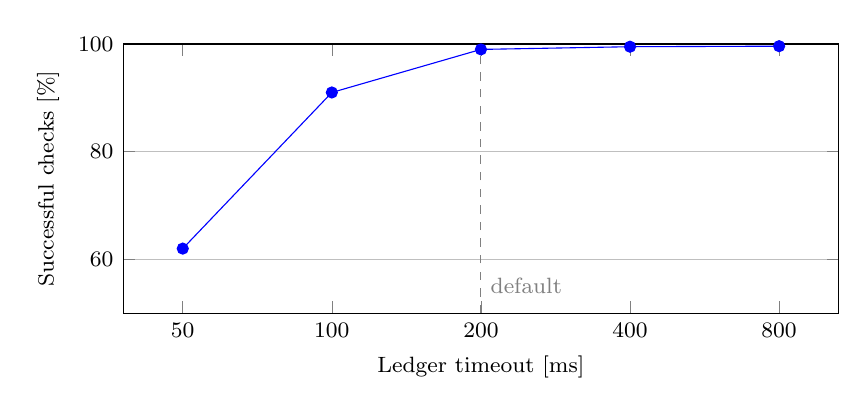
\begin{tikzpicture}
      \begin{axis}[width=0.88\linewidth, height=50mm, xlabel={Ledger timeout [ms]}, ylabel={Successful checks [\%]}, xmode=log, log basis x=2, xtick={50,100,200,400,800}, xticklabels={50,100,200,400,800}, ymin=50, ymax=100, ymajorgrids, font=\footnotesize]
        \draw[dashed, gray] (axis cs:200,50) -- (axis cs:200,100) node[pos=0.1, right, font=\footnotesize] {default};
        \addplot[mark=*, blue] coordinates {(50,62) (100,91) (200,99) (400,99.5) (800,99.6)};
      \end{axis}
    \end{tikzpicture}
    \caption{Sensitivity to the ledger timeout, around its default.}\label{fig:guide:robustness-sensitivity}
  \end{subfigure}
  \caption{Robustness: the registry during a node failure and under changes to its main parameter.}
  \label{fig:guide:robustness}
\end{figure}

\subsection{Threats to validity}\label{app:chapters:validity}
\guidebeat{what could make the results wrong or not generalise, and what was done about each}{the mitigations}{whether the example is representative of real use}{related work}
For the registry, the issuer sets are synthetic and all measurements used one machine. For each threat, describe what you did to address it and what remains unresolved.

%----------------------------------------------------------------------------
\section{Related work and gap analysis}\label{app:chapters:related}
%----------------------------------------------------------------------------
\textbf{Criteria B/2 (0--4) and D/1 (0--5).} Place related work after the evaluation so comparisons can refer to results the reader has already seen.
\textbf{Novelty:} plot related work in a positioning figure, compare the closest approaches against requirements in a gap matrix, and state the gap only your work fills.
\textbf{Relevance:} include current industrial solutions and recent research to show that the gap remains open.

\textbf{In the sheet's words.} One step below the top of B/2 (\cref{app:tdk:sheet}), \enquote{2: újszerű ipari megoldások vagy közismert kutatási eredmények} is where a chapter without recent research lands. D/1 falls to \enquote{1--2: ismert (a kutatási terület szakirodalomban számos megoldás ismert a tárgyalt problémára, és ezek „másolás jellegű” alkalmazására került sor a dolgozatban)}, or to the incremental step quoted in \cref{app:tdk:sheet}, when the gap matrix shows a close neighbour; argue the difference here.

\subsection{Comparison criteria}\label{app:chapters:comparison-criteria}
Compare approaches against the introduction's requirements, here \cref{req:guide:timely,req:guide:offline,req:guide:private}. Add other criteria, such as maturity or license, only when readers need them.

\subsection[Existing approaches]{Existing approaches\skimmark}\label{app:chapters:existing-approaches}
\guidebeat{how each family of approaches works and where it falls short}{citations, the positioning figure and the gap matrix}{what each approach does with the example}{the gap}
Group related work into families and compare each against the requirements. Use \cref{fig:guide:positioning} to separate approaches by two main properties, leaving the gap as an empty cell. Then compare the closest approaches requirement by requirement in \cref{tab:guide:related}. The matrix alone should show the gap as the one column meeting every row.

In the positioning figure, plot related work as dots on two axes with three levels each. Put a star for your work in the cell no existing approach reaches. Draw an arrow from the closest approach and label what you add. Choose the two properties that best distinguish approaches, either individual requirements or summaries of several. Give levels specific names, not low, medium and high.
\begin{runningexample}[elsewhere]
With Approach C, the closest one, the employer checks offline against a list fetched in the morning, so a diploma revoked at noon passes every check until the next fetch: it fails \cref{req:guide:timely}.
\end{runningexample}

\begin{figure}[!ht]
  \centering
  \begin{tikzpicture}[
      work/.style={circle, fill=gray!60!black, draw=white, line width=0.5pt, inner sep=0pt, minimum size=2.3mm},
      wlbl/.style={anchor=west, font=\footnotesize, inner sep=1pt, fill=white},
      wnote/.style={anchor=north west, font=\footnotesize\itshape, text=gray!70!black, inner sep=1pt, fill=white},
      tick/.style={font=\footnotesize\bfseries, align=center},
      sub/.style={font=\footnotesize\itshape, text=gray!80!black, align=center}]
    \def\cA{1.8}\def\cB{6.0}\def\cC{10.2} % columns: the levels of the second property
    \def\rA{0.9}\def\rB{2.6}\def\rC{5.0}  % rows: the levels of the first property
    \def\xmax{14.6}\def\ymax{6.1}
    \fill[blue!8, rounded corners=4pt] ({(\cB+\cC)/2},\rC-0.75) rectangle (\xmax,\ymax-0.15); % the gap
    \foreach \y in {\rA,\rB,\rC} \draw[gray!30, dashed] (0,\y) -- (\xmax,\y);
    \foreach \x in {\cA,\cB,\cC} \draw[gray!30] (\x,0) -- (\x,\ymax-0.15);
    \draw[line width=0.9pt, -{Stealth[length=2.6mm]}] (0,0) -- (\xmax+0.3,0);
    \draw[line width=0.9pt, -{Stealth[length=2.6mm]}] (0,0) -- (0,\ymax+0.2);
    \node[anchor=south west, inner sep=0pt, font=\footnotesize] at (0.15,\ymax+0.05)
      {\textbf{How soon a revocation is seen} $\uparrow$\enspace\textit{how far an approach meets \cref{req:guide:timely}}};
    \node[anchor=north east, align=right, font=\footnotesize] at (\xmax+0.3,-0.85)
      {\textbf{What a check needs} $\rightarrow$\\\textit{how far it meets \cref{req:guide:offline}}};
    \foreach \y/\name/\what in {\rC/within $\delta$/bounded by\\the clocks, \rB/minutes/a cache's\\lifetime, \rA/days/the next list} {%
      \draw (-0.08,\y) -- (0.08,\y);
      \node[tick, anchor=south east] at (-0.15,\y+0.02) {\name};
      \node[sub, anchor=north east] at (-0.15,\y+0.02) {\what};
    }
    \foreach \x/\name/\what in {\cA/the issuer/asked at every check, \cB/a fresh list/fetched before the check, \cC/nothing/the credential alone} {%
      \draw (\x,-0.08) -- (\x,0.08);
      \node[tick, anchor=north] at (\x,-0.15) {\name};
      \node[sub, anchor=north] at (\x,-0.5) {\what};
    }
    \node[work] (a) at (\cA,\rC) {};
    \node[wlbl] at (a.east) {Approach A};
    \node[wnote] at (\cA+0.05,\rC-0.2) {online status checks};
    \node[work] (d) at (\cB,\rB) {};
    \node[wlbl] at (d.east) {Approach D};
    \node[work] (b) at (\cC,\rA) {};
    \node[wlbl] at (b.east) {Approach B};
    \node[work] (c) at (\cC,\rB) {};
    \node[wlbl] at (c.east) {Approach C};
    \node[wnote] at (\cC+0.05,\rB-0.2) {the closest approach};
    % this work, reached from the closest approach
    \draw[blue!60!black, line width=1.2pt, dashed, -{Stealth[length=2.6mm]}] (c.north) -- (\cC,\rC-0.32);
    \node[star, star points=5, star point ratio=2.3, minimum size=6.5mm, inner sep=0pt,
          fill=blue!60!black, draw=white, line width=0.6pt] (tw) at (\cC,\rC) {};
    \node[anchor=west, font=\normalsize\bfseries, text=blue!60!black, inner sep=1pt] at ([xshift=2pt]tw.east) {This work};
    \node[anchor=north west, font=\footnotesize\itshape, text=blue!60!black, inner sep=1pt, align=left] at (\cC+0.38,\rC-0.22) {a registry with\\bounded staleness};
    \node[anchor=west, font=\footnotesize, text=blue!60!black, align=left, inner sep=1pt] at (\cC+0.2,3.35)
      {+ values fresh within $\delta$\\+ checked without the issuer};
  \end{tikzpicture}
  \caption{Approaches compared on two distinguishing properties. Grey dots mark existing approaches; the blue star marks this work in the previously empty cell. The dashed arrow from the closest approach identifies what this work adds.}
  \label{fig:guide:positioning}
\end{figure}

\begin{table}[!ht]
  \centering
  \caption{Gap matrix: each requirement against the closest approaches. \gaplegend. Cells for this work point to the evaluation result that backs them.}
  \label{tab:guide:related}
  \renewcommand{\arraystretch}{1.3}
  % Every column but the requirement's has a fixed width and wraps, so a long cell grows downwards
  % instead of squeezing the requirement column under its heading.
  \begin{tabularx}{\linewidth}{>{\raggedright\arraybackslash}p{3.2em} >{\raggedright\arraybackslash}X *{3}{>{\centering\arraybackslash}p{5.5em}} >{\centering\arraybackslash}p{6.5em}}
    \toprule
    & \textbf{Requirement} & \textbf{Approach A} & \textbf{Approach B} & \textbf{Approach C} & \textbf{This work} \\
    \midrule
    \ref{req:guide:timely}  & Timely revocation & \gapyes & \gapno  & \gappartial & \gapyes\,(\cref{thm:guide:stale}) \\
    \ref{req:guide:offline} & Offline checks    & \gapno  & \gapyes & \gapyes     & \gapyes\,(\cref{rq:guide:correct}) \\
    \ref{req:guide:private} & Holder privacy    & \gapno  & \gapyes & \gappartial & \gapyes\,(\cref{rq:guide:correct}) \\
    \bottomrule
  \end{tabularx}
\end{table}

\subsection{Gap}\label{app:chapters:gap}
\guidebeat{the gap in one sentence, closed by this work}{the gap matrix and the results of the evaluation}{the scenario as the case only this work handles}{the conclusion}
State the gap in one sentence, supported by the positioning figure and matrix. In the same paragraph, cite evaluation results showing that your work closes it. This establishes novelty. Here, the gap is revocation visible within $\delta$ to a verifier that asks nobody; the registry provides it according to \cref{thm:guide:stale} and the measurements for \cref{rq:guide:correct}.

%----------------------------------------------------------------------------
\section{Conclusion and future work}\label{app:chapters:conclusion}
%----------------------------------------------------------------------------
\textbf{Criterion E.} Show that you delivered and evaluated the contributions promised in the introduction. Readers often open the conclusion just after the abstract, so start with the achievements. End with limitations and concrete future work.
\textbf{Novelty:} restate each contribution from the introduction with the gap it closes.
\textbf{Correctness:} restate each with the proof or measurement behind it.

\subsection[Summary]{Summary\skimmark}\label{app:chapters:summary}
\guidebeat{each contribution and its evidence}{the chapters behind C1--C3}{the example, now solved}{the limitations}
Write one paragraph per contribution with its evidence: \cref{c:guide:model} with \cref{thm:guide:stale}, \cref{c:guide:registry} with the archived artifact, and \cref{c:guide:eval} with answers to \cref{rq:guide:correct,rq:guide:scale,rq:guide:robust}. Close the introductory scenario in a one- or two-sentence box.
\begin{runningexample}[in retrospect]
The withdrawn diploma no longer gets anyone hired: the employer's offline check rejects it within $\delta$ of its revocation, and the university never learns that the employer asked.
\end{runningexample}

\subsection[Limitations and future work]{Limitations and future work\skimmark}\label{app:chapters:future}
\guidebeat{what is still open, and the next step that would lift each limitation}{the threats to validity}{what the example does not cover}{the venue to target next}
Tag each limitation so future work can refer to the one it addresses.
\begin{limitations}
  \item\label{lim:guide:synthetic} \textbf{Synthetic workloads.} The evaluation uses synthetic issuer sets only.
  \item\label{lim:guide:force} \textbf{No forced revocation.} The registry cannot make an issuer revoke a credential it should.
\end{limitations}
